\documentclass[]{article}

\usepackage{amsmath}
\usepackage{amssymb}
\usepackage{graphicx}
\usepackage{float}
\usepackage{multicol}
\usepackage{fancyhdr}
\fancyhead[L, CO] {}
\fancyhead[C, CO] {AdvContr - Résumé 2022}
\fancyhead[R, CO] {}
\usepackage[margin=1.5cm,landscape]{geometry}
\pagestyle{fancy}
\usepackage{mathtools} % for '\splitdfrac' macro
\usepackage[dvipsnames]{xcolor}
\usepackage{subfiles}
\usepackage{mdframed}

\def\Pcolor{\textcolor{RoyalBlue}}
\def\Icolor{\textcolor{OrangeRed}}
\def\Dcolor{\textcolor{ForestGreen}}
\def\Ucolor{\textcolor{Orange}}
\def\bcolor{\textcolor{RubineRed}}
\def\acolor{\textcolor{BlueViolet}}


\begin{document}
\begin{multicols}{3}
\subfile{fonction_transfert}
\subfile{espace_etats}
\subfile{regulateurs}
\subfile{nyquist}
\subfile {observateur}
\subfile{autres}
\end{multicols}
\pagebreak
\begin{center}
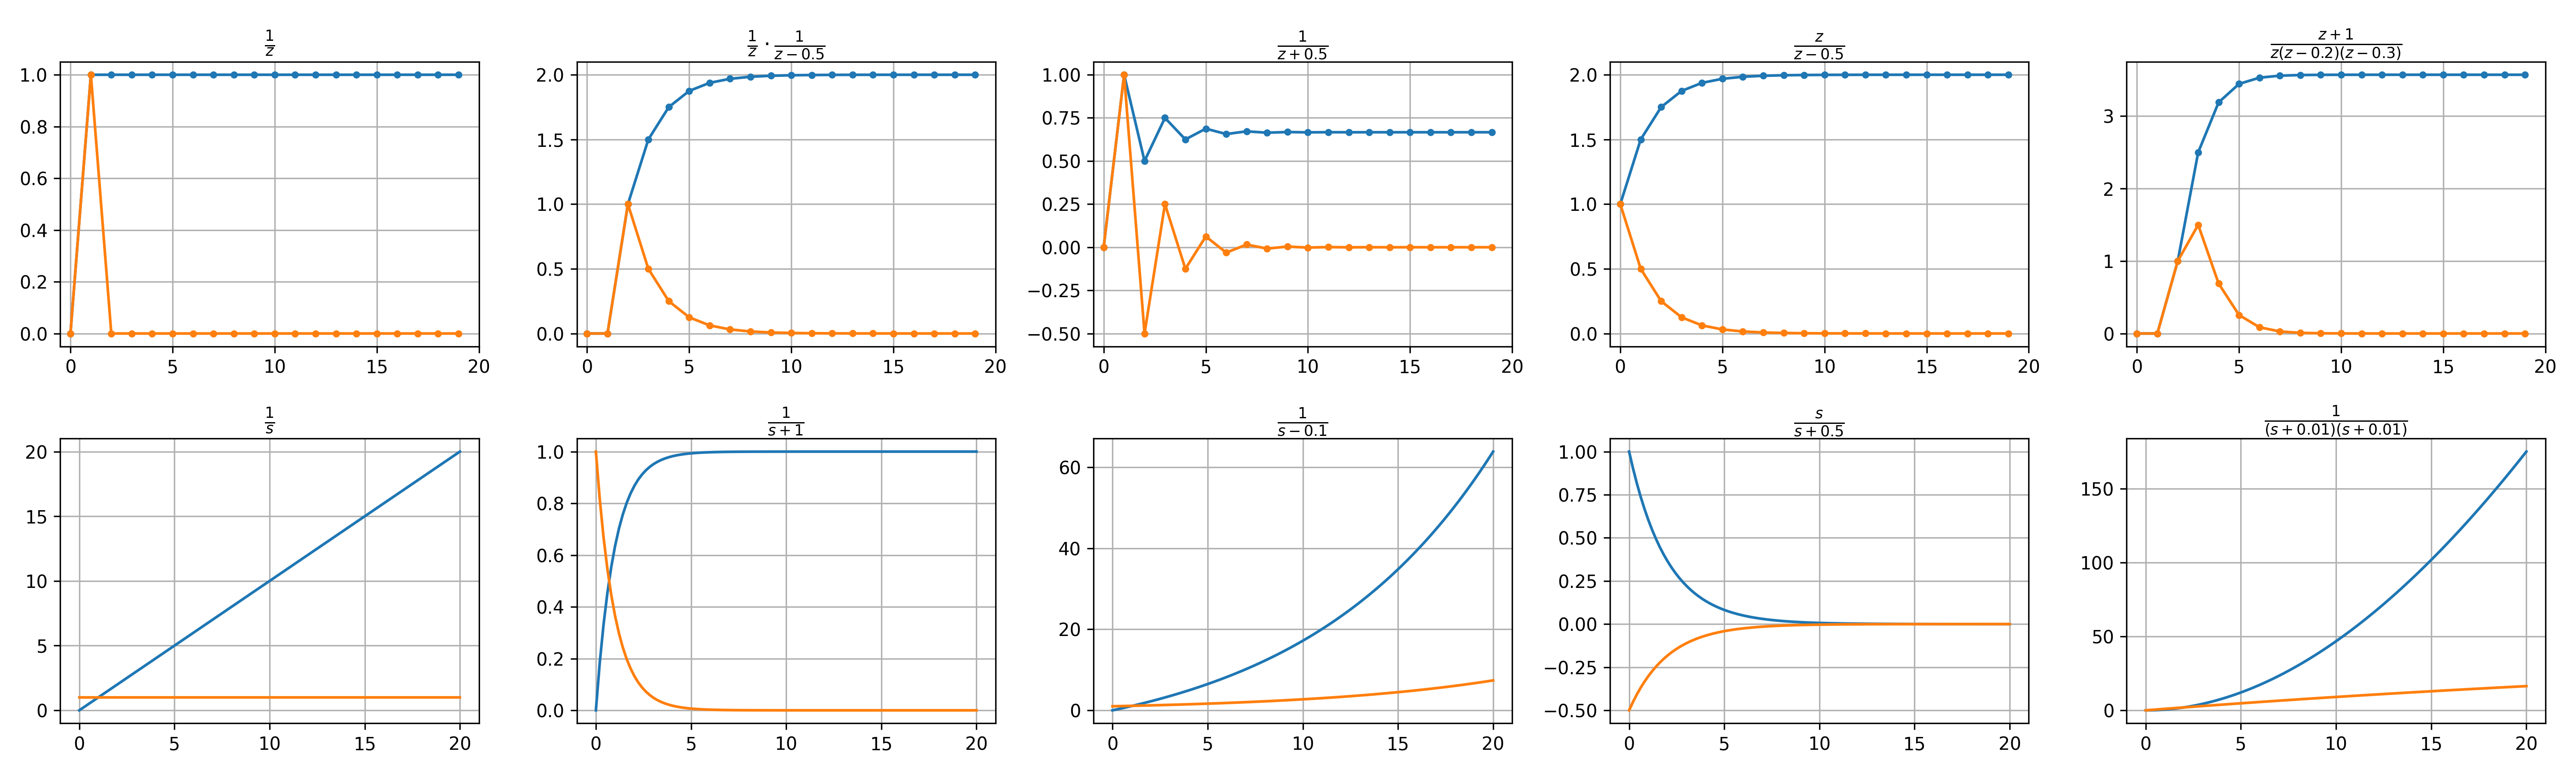
\includegraphics[width=\textwidth]{Allures.png}
\end{center}


\section{A trier}
\subsection{Identification}
Avec deux bodes, on peut identifier lequel est $G(s)$ et lequel est $\frac{1}{G(s)}$ en regardant une valeur (en dB) de $x$ qui devient $-x$



\end{document}